\documentclass{article} % For LaTeX2e
\usepackage{nips12submit_e,times}
%\documentstyle[nips12submit_09,times,art10]{article} % For LaTeX 2.09

% For figures
\usepackage{multirow}

\usepackage{graphicx} % more modern
%\usepackage{epsfig} % less modern
\usepackage{subfigure} 

% For citations
\usepackage{natbib}
\usepackage{subfigure}
% For algorithms
\usepackage{algorithm}
\usepackage{algorithmic}

% As of 2011, we use the hyperref package to produce hyperlinks in the
% resulting PDF.  If this breaks your system, please commend out the
% following usepackage line and replace \usepackage{icml2013} with
% \usepackage[nohyperref]{icml2013} above.
\usepackage{hyperref}
\nocite{*}

% Packages hyperref and algorithmic misbehave sometimes.  We can fix
% this with the following command.
\newcommand{\theHalgorithm}{\arabic{algorithm}}

% jovo added stuff
\newcommand{\iid}{\overset{iid}{\sim}}
\newcommand{\mbX}{\mathbf{X}}
\newcommand{\mbY}{\mathbf{Y}}
\newcommand{\Real}{\mathbb{R}}
\providecommand{\mh}[1]{\hat{#1}}
\providecommand{\mb}[1]{\boldsymbol{#1}}
\providecommand{\mc}[1]{\mathcal{#1}}
\newcommand{\from}{{\ensuremath{\colon}}}           % :
\usepackage{amsmath,amssymb,amsfonts}

\newcommand{\efoo}{\end{footnotesize}}
\newcommand{\bfoo}{\begin{footnotesize}}


% Employ the following version of the ``usepackage'' statement for
% submitting the draft version of the paper for review.  This will set
% the note in the first column to ``Under review.  Do not distribute.''

% Employ this version of the ``usepackage'' statement after the paper has
% been accepted, when creating the final version.  This will set the
% note in the first column to ``Proceedings of the...''
% \usepackage[accepted]{icml2013}

% jovo additions
\usepackage{color}
\newcommand{\jovo}[1]{{\color{magenta}{\it JoVo says: #1}}}
% \newcommand{\Real}{\mathbb{R}}
\usepackage{color}
\newcommand{\francy}[1]{{\color{blue}{\it Fra says: #1}}}
\newtheorem{theorem}{Theorem}%[section]
\newtheorem{lemma}[theorem]{Lemma}
\newtheorem{proposition}[theorem]{Proposition}
\newtheorem{corollary}[theorem]{Corollary}
\newtheorem{result}[theorem]{Result}
\newtheorem{definition}[theorem]{Def}


% The \icmltitle you define below is probably too long as a header.
% Therefore, a short form for the running title is supplied here:
\title{Multiresolution dictionary learning for conditional distributions}


%\nipsfinalcopy % Uncomment for camera-ready version

\begin{document}


\maketitle



\section{Simulation studies}\label{section:simulation}

In order to assess the predictive performance of the proposed model, different simulation scenarios were considered. Let $n$ be the number of observations, $y \in \Re$ the response variable and $x \in \Re^p$ a set of predictors. The Gibbs sampler was run considering $20,000$ as the maximum number of iterations with a burn-in of $1,000$. Gibbs sampler chains were stopped testing normality of normalized averages of functions of the Markov chain \cite{Chauveau98anautomated}. Parameters $(a,b)$ and $\alpha$ involved in the prior density of parameters $\sigma_{B_j}$s and $V_{B_j}$s were set respectively equal to $(3,1)$ and $1$.

In all simulation scenarios, predictors were assumed to lie close a $r$-dimensional space, either a lower dimensional plane or a non linear manifold, with $r<<p$. For each synthetic dataset, the proposed model was compared with CART and lasso in terms of mean squared error. Mean squared errors were computed based on leave-one=out predictions. For CART and Lasso standard Matlab packages were utilized and the regularization parameter of Lasso was chosen based on  the AIC. The supplementary material includes more results about experiments involved in this section.

\subsection{Illustrative Example}
First let us consider the simple toy example of \S \ref{section:setting}. We created an equally spaced grid of points $t_i=0, \ldots, 20$. Then, we let $\eta_i=\sin(t_i)$ and predictors be a linear function of $\eta_i$ plus Gaussian noise, i.e. $x_{ij}=\eta_i + \epsilon_{ij}$ with $\epsilon_{ij} \sim N(0,0.1)$ for $j\in \{1, \ldots, p \}$. In particular, we set $p=1,000$. The response was drawn from the following mixture of Gaussians
\begin{equation}
y_i \sim w_i \mathcal{N}(-2,1) + (1-w_i) \mathcal{N}(2,1) 
\end{equation}
with $w_i=|\eta_i|$.  Figure \ref{plotDensity} shows the estimated density of two data points. These estimates were obtained by performing leave-one-out prediction for different number of observations in the training set. As the figure clearly shows our construction facilitates an estimate of the density $y$ that become closer to the true density as the number of observations in the training set increases.


\begin{figure}[h!]
\centering
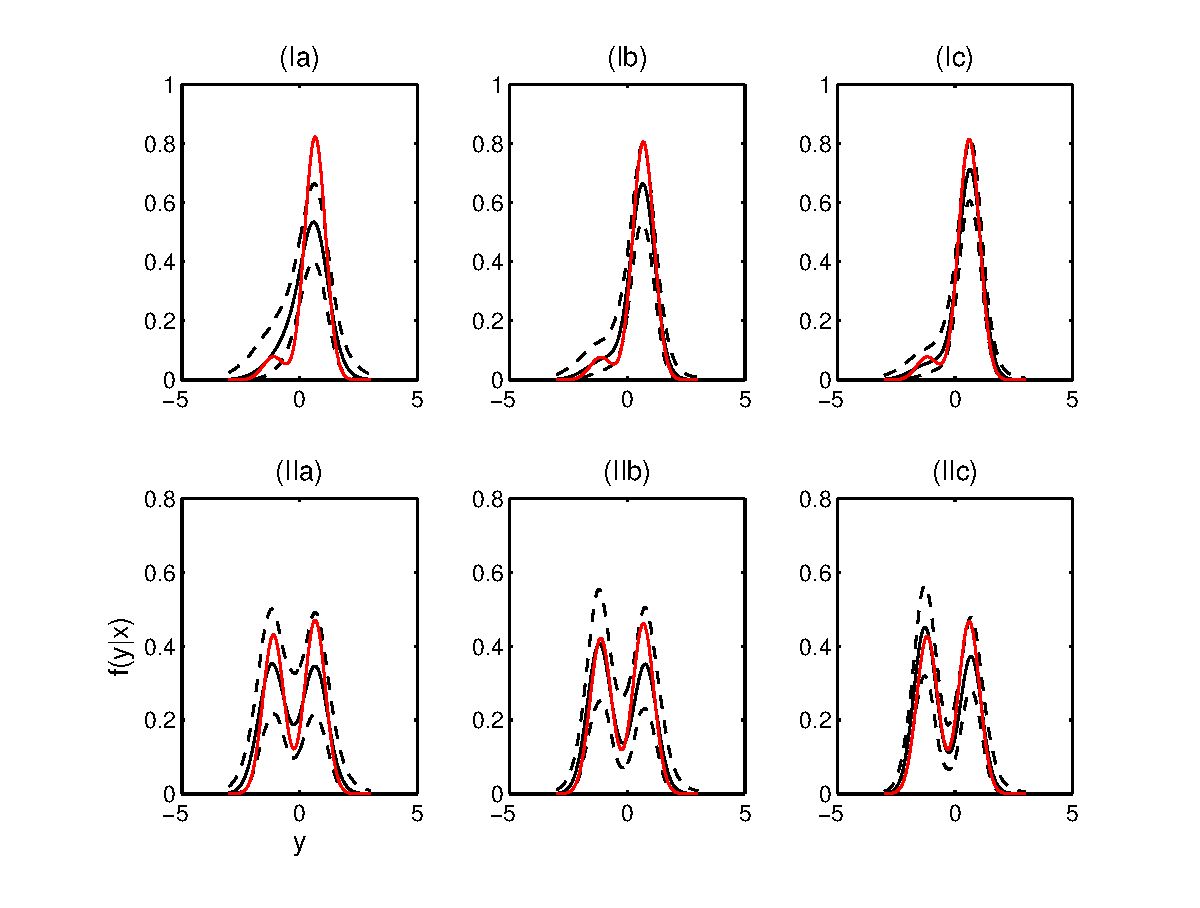
\includegraphics[width=120mm,height=70mm]{ch3_density.eps}
% 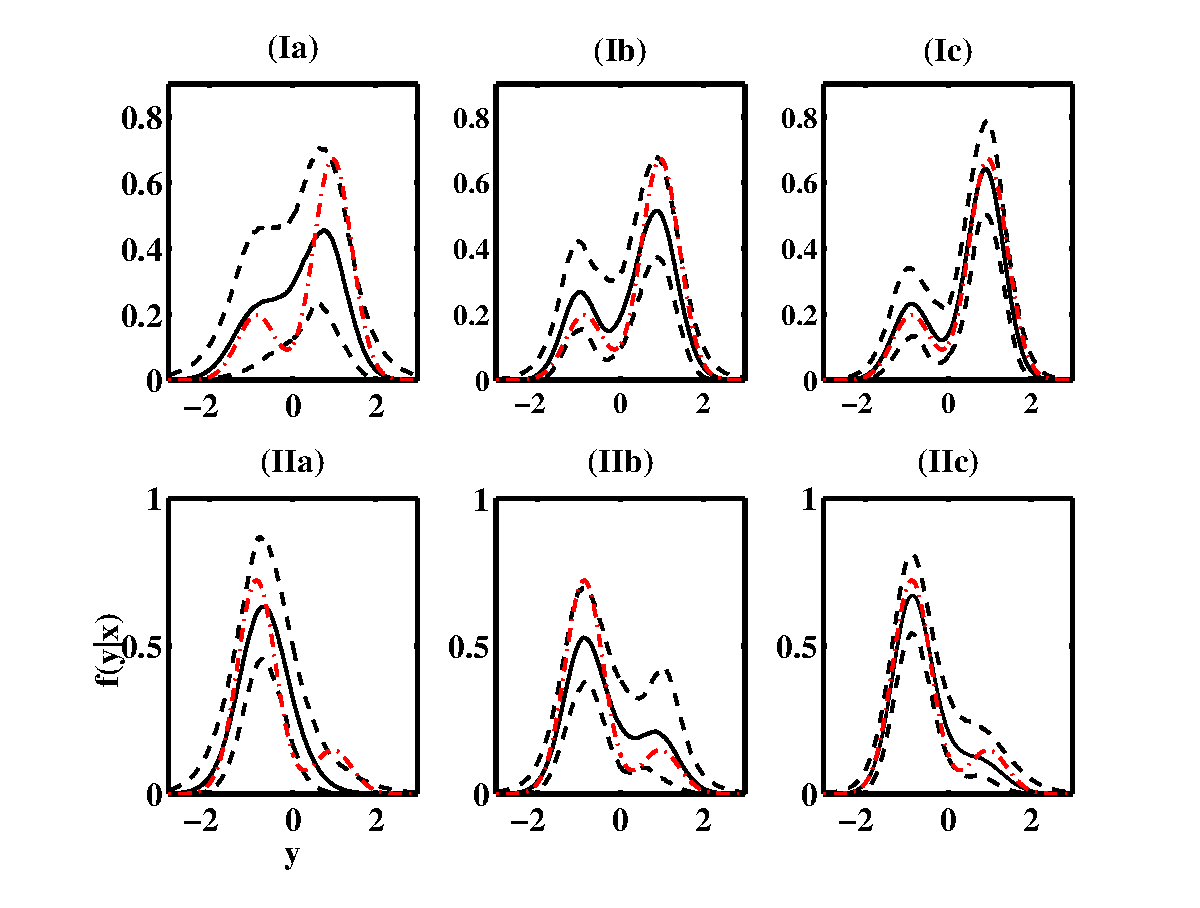
\includegraphics[width=90mm,height=80mm]{densityestimate.eps}
\caption{Illustrative example: Plot of true (red dashed-dotted line) and estimated ($50$th percentile: solid line, $2.5$th and $97.5$th percentiles: dashed lines) density for two data points $(I, II)$ considering different training set size (a:100, b:150, c:200). } \label{plotDensity}
\end{figure}


%% INSERT  For each resolution level, the new observation was allocated to the set with closer center. 

\subsection{Linear lower dimensional space} \label{section:linear}


In this section, predictors and response were assumed to lie close to a lower dimensional plane. In practice, we modeled $z_i=(y_i,x_i^t)^t$ through the following factor model

\begin{equation} z_i=\Lambda \eta_i + \epsilon_i \end{equation} 
with $\epsilon_i \sim \mc{N}(0,\Sigma_0)$, $\Sigma_0=diag(\sigma_1, \ldots, \sigma_p)$, $\Lambda$ being a $p \times r$ matrix, $\eta_i \sim \mc{N}(0,I)$ and $r<<p$. The loading matrix was derived as the product of a matrix with orthogonal columns and a diagonal matrix with positive elements on the diagonal, i.e. $\Lambda=\Gamma \Theta$. In particular, the columns of $\Gamma$ were uniformly sampled from the Stiefel manifold while the diagonal matrix of $\Theta$ were sampled from an inverse Gamma with shape and rate parameters $(1,4)$. We set $r=5$.

As measure of comparison we adopted the ratio between cpu times and the ratio between mean squared errors. Define $t_{m}^{\ell}$ as $$t_{m}^{\ell}=m(MSB)/m(\ell)$$
where $m$ is either CPU time expressed in seconds or mean squared errors, MSB is our approach and $\ell$ is the competitor. For each simulation scenario, we sampled $M$ datasets so that $M$ values of $t_{m}^{\ell}$ were obtained. We sampled $M=20$ datasets involving $100$ observations and for each method we performed leave-one-out predictions. Figure \ref{boxplot:linear}(I) shows boxplots of $t_{mse}^{\ell}$ as $p$ increases. Clearly, our method outperforms the competitors in terms of mean squared errors. Furthermore, as shown in figure \ref{boxplot:linear}(II), our approach can scale substantially better than competitors to huge dimensions of the predictor space. 

%
%In this section, the vector of predictors was assumed to lie close to a lower dimensional plane. In practice,  predictors were modeled through a factor model as follows 
%\begin{equation} x_i=\Lambda \eta_i + \epsilon_i \end{equation} 
%with $\epsilon_i \sim \mc{N}(0,\Sigma_0)$, $\Sigma_0=diag(\sigma_1, \ldots, \sigma_p)$, $\Lambda$ being a $p \times r$ matrix, $\eta_i \sim \mc{N}(0,I)$ and $r<<p$. The loading matrix was derived as the product of a matrix with orthogonal columns and a diagonal matrix with positive elements on the diagonal, i.e. $\Lambda=\Gamma \Theta$. In particular, the columns of $\Gamma$ were uniformly sampled from the Stiefel manifold while the diagonal matrix of $\Theta$ were sampled from an inverse Gamma with shape and rate parameters $(1,4)$. In the first simulation scenario, the vector $x$ and $y$ were jointly sampled from the above factor model.  In the second simulation scenario, $x$ was sampled from the above factor model while $y$ was sampled from a normal with location and scale parameter $(1,1)$ if the first variable was positive, i.e. $x_1>0$, and from a normal with location and scale $(-1,1)$ otherwise. 
%
%Define $t_{mse}^{\ell}$ as the the ratio between mean squared errors under MSB and method $\ell$. We sampled $M=20$ datasets from each simulation scenario so that $M$ values of $t_{mse}^{\ell}$ were obtained for each simulation scenario.   Figure \ref{boxplot:linear}(I) shows boxplots of these ratios considering lasso and Cart as competitors as $p$ increases. Clearly, our method outperforms the competitors in terms of mean squared errors under both simulation scenarios. Figure \ref{boxplot:linear}(II) shows that our model can scale substantially better than competitors to large $p$. Table  \ref{table:linear2} show mean squared errors under the second simulation scenario. As shown, in almost all experiments, our model is able to perform as well as or better than the model associated to the lowest mean squared error.
%
\begin{figure}
\centering
\begin{tabular}{ll}
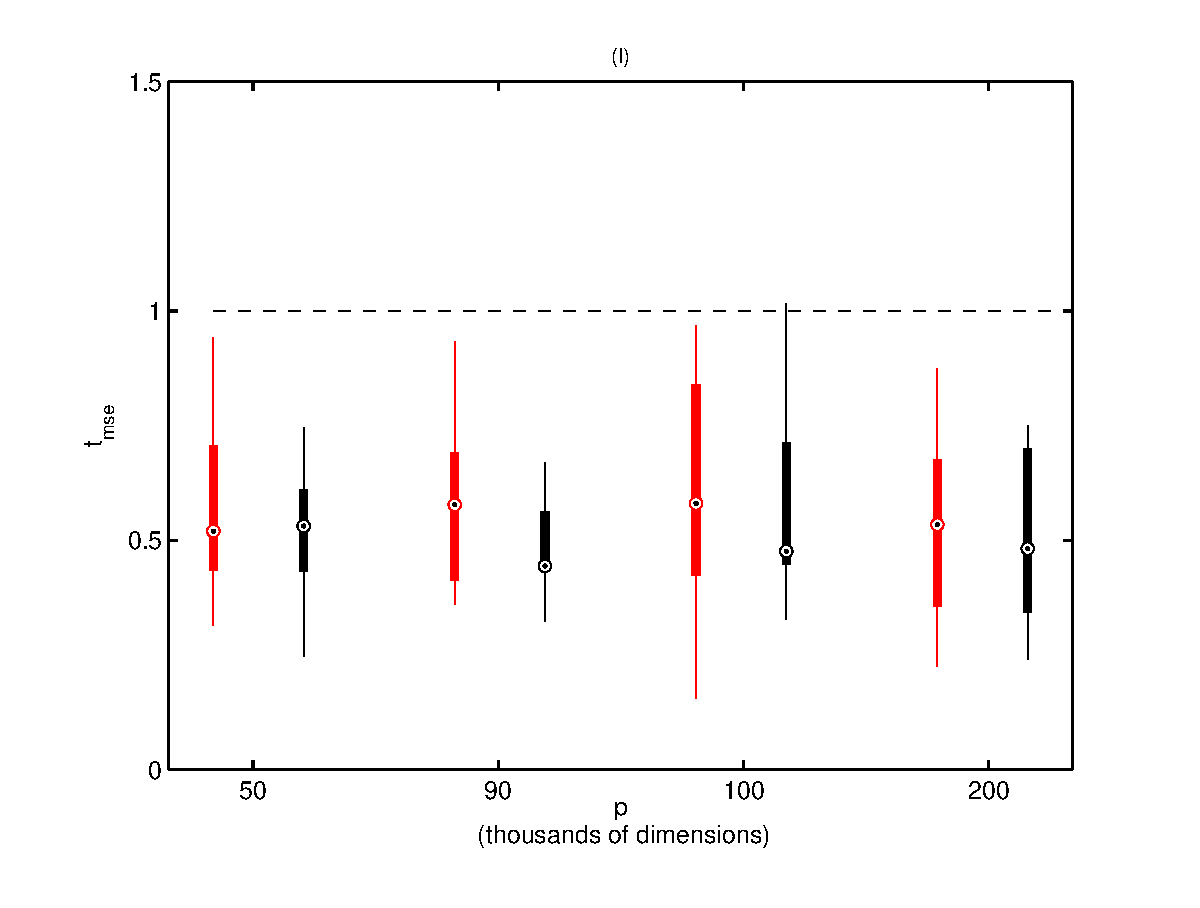
\includegraphics[width=70mm,height=50mm]{boxplot_exp1.eps} &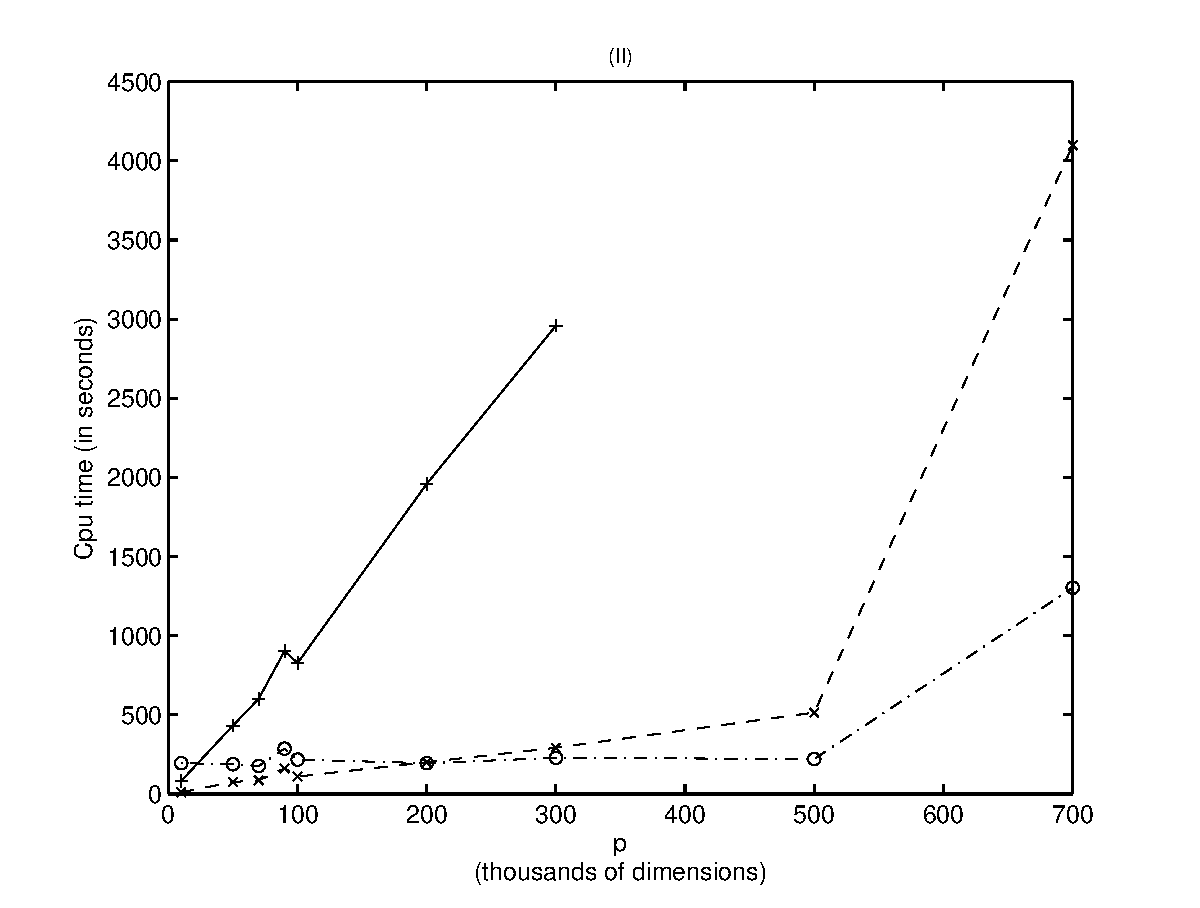
\includegraphics[width=70mm,height=60mm]{cpuTime_exp1.eps}
% 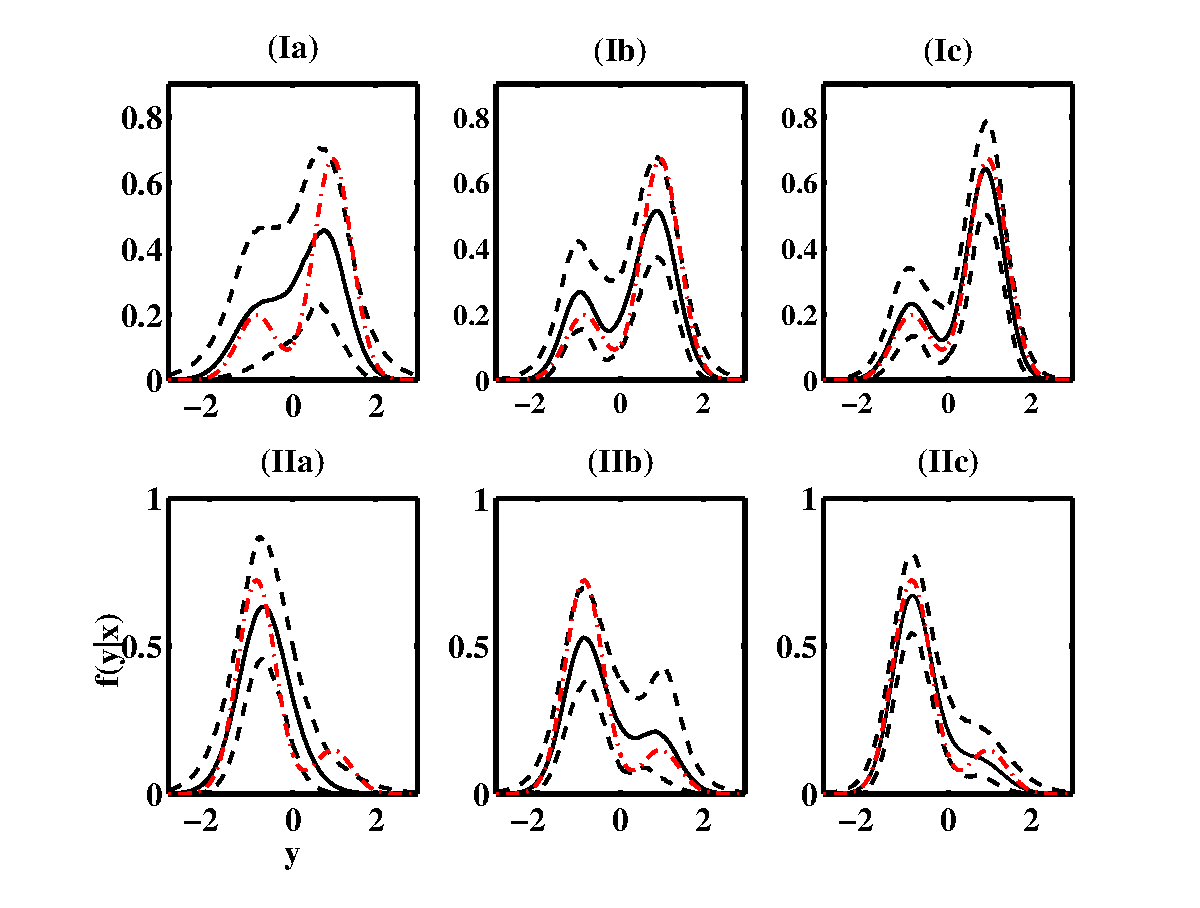
\includegraphics[width=90mm,height=80mm]{densityestimate.eps}

\end{tabular}
\caption{(I) Boxplots of $t_{mse}$ as $p$ increases. (II) Plot of Cpu time (in seconds) for Lasso (dash), Cart (solid) and MSB (dash-dot) under the first simulation scenario} \label{{boxplot:linear}}

\end{figure}


\subsection{Non-Linear lower dimensional space}

In this section predictors were assumed to lie close to a lower dimensional non-linear manifold. In the first simulation study, predictors and response were jointly sampled from an $N$ components mixture of factor analyzers. For each mixture components, the loading matrix and variances were sampled as in \S \ref{section:linear}, while mixture weights were sampled from a $Dirichlet(1, \dots, 1)$. The number of latent factors was considered to be increasing in the number of components. In practice, we let the $h$th mixture component be modeled through $h$ factors. We set $N=5$ (the supplementary material shows results for different numbers of mixture components). In the other simulation scenario predictors were assumed to lie close to the Swissroll manifold (see figure 1 in the supplementary material), a two dimensional manifold embedded in $\Re^p$ while the response was sampled from a normal with mean equal to one coordinate of the manifold and standard deviation one.

For both data scenarios, we sampled $M=20$ datasets involving $100$ observations and we performed leave-one-out predictions. Figure \ref{MFA:plot}(I) and  \ref{swiss:plot}  show boxplots of mean squared errors as $p$ increases.  Again our model is associated to better predictive performance compared to Cart and lasso. To show how the performance of our model varies for different sample sizes,  we sampled datasets involving different number of observations. In practice, the dimension of the predictor space was considered fixed, i.e. $p=300,000$ and ratios $t_{cpu}(\ell)$ were computed considering sample sizes $n \in \{100,200,300 \}$. As shown in figure \ref{MFA:plot}(II), the  gap between our model and competitors improves as $n$ increases. 


%
%Figure \ref{MFA:plot} and \ref{swiss:plot}  mean squared errors based on leave-one-out predictions considering each of the three simulation scenario. 
%
%\begin{figure}
%\centering
%\begin{tabular}{cc}
%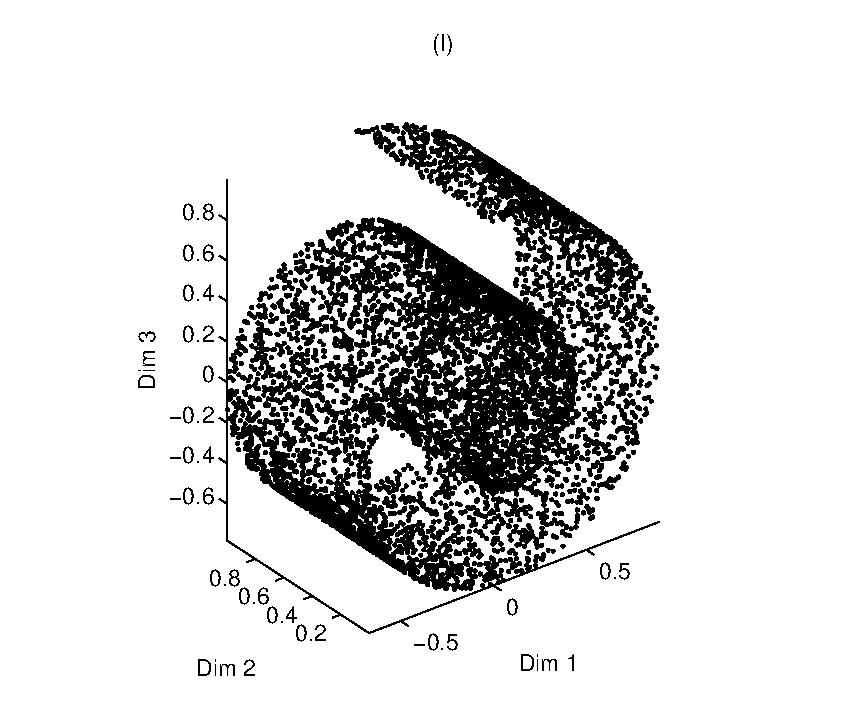
\includegraphics[width=60mm,height=50mm]{Swissroll.eps} & 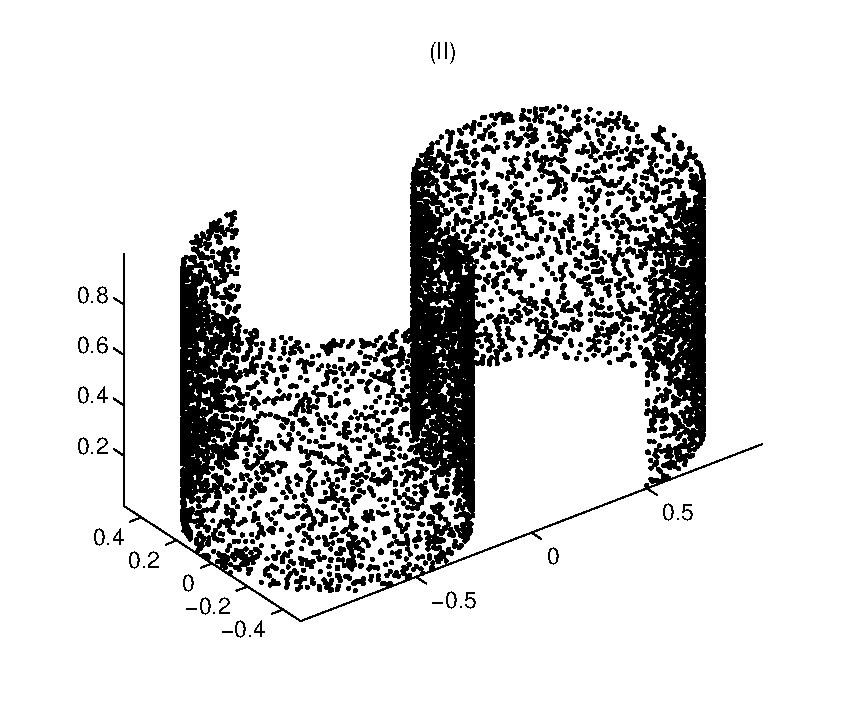
\includegraphics[width=60mm,height=50mm]{SManifold.eps}
%\end{tabular}
%\caption{Non-linear manifolds: Swissroll (I) and S-Manifold (II) embedded in $\mathcal{R}^3$} \label{manifold:nonlinear}
%\end{figure}


\begin{figure}[h!]
\centering
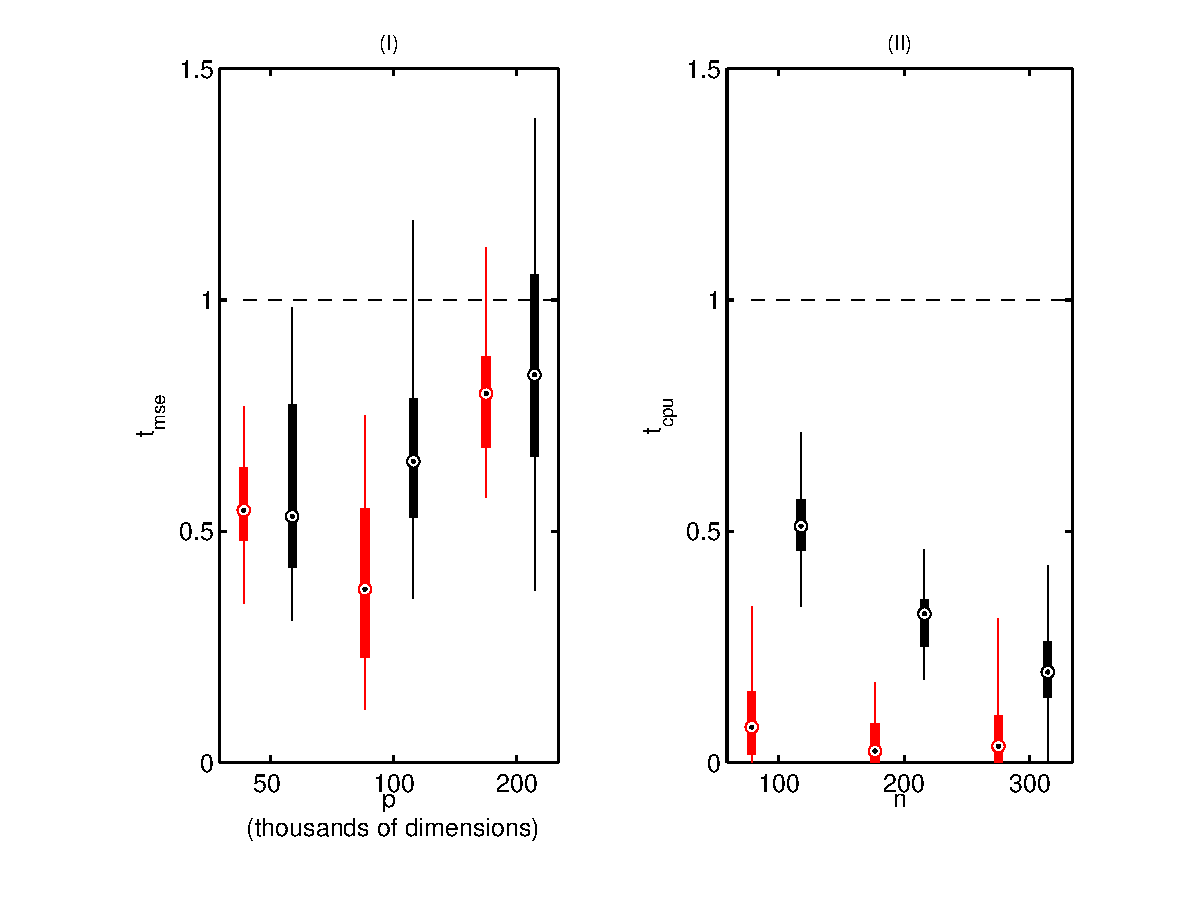
\includegraphics[width=140mm,height=60mm]{boxplot_MFA.eps} 
\caption{Boxplots of (I) $t_{mse}$  as $p$ increases and (II) $t_{cpu}$ for a fixed $p=300,000$ and different sample sizes under data drawn from a mixture of factor analyzers} \label{MFA:plot}
% 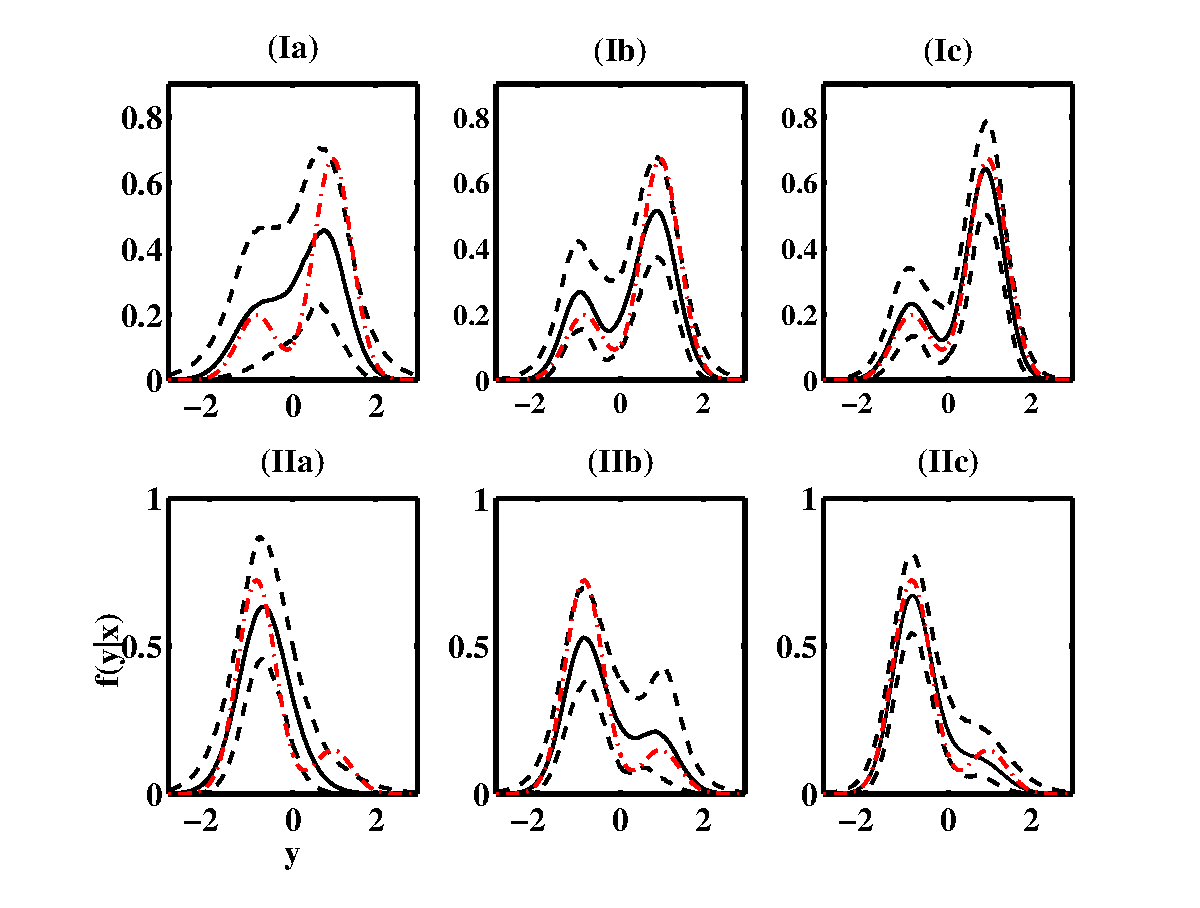
\includegraphics[width=90mm,height=80mm]{densityestimate.eps}
\end{figure}


\begin{figure}
\centering
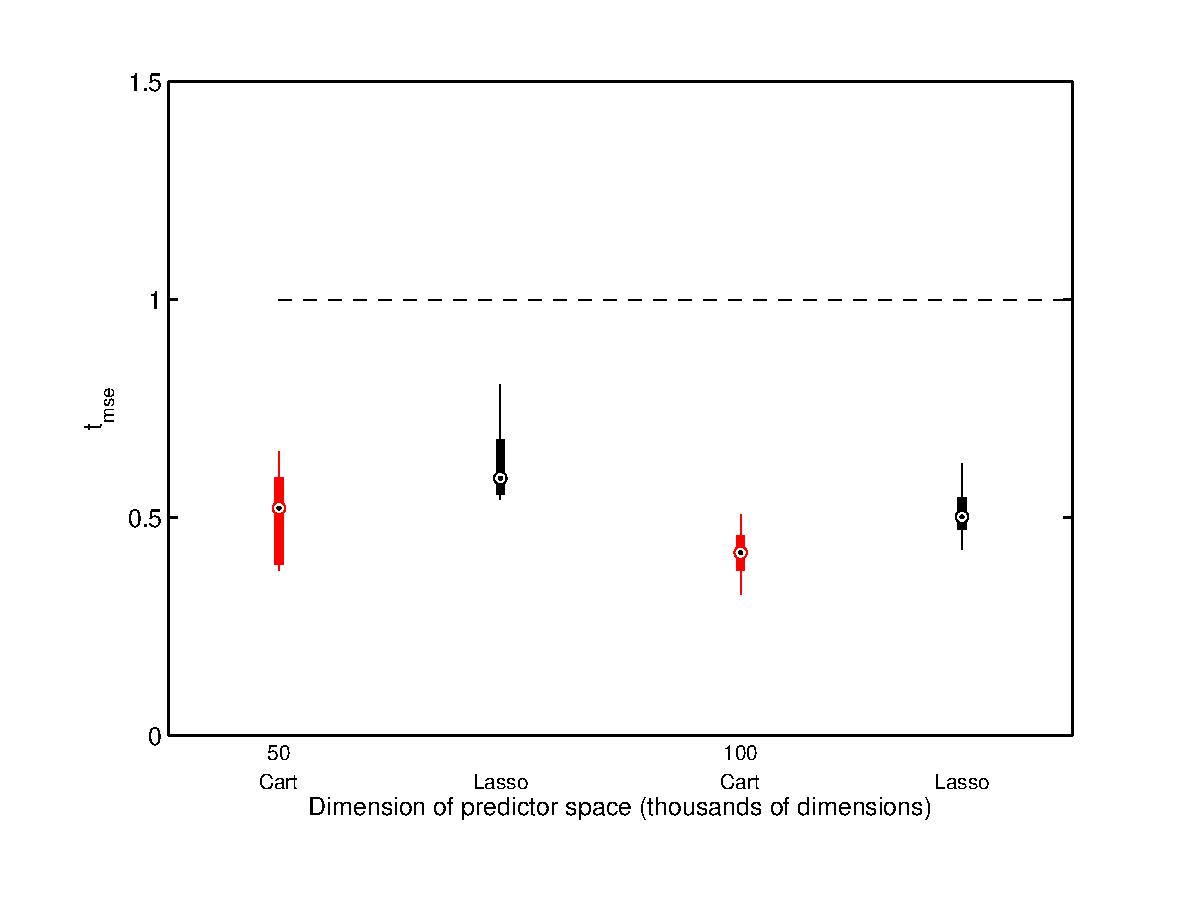
\includegraphics[width=120mm,height=60mm]{box_exp3.eps} 
\caption{Boxplots of  $t_{mse}$ as $p$ increases under the swiss roll simulation scenario} \label{swiss:plot}
\end{figure}



\section{Real application}

We assessed the predictive performance of the proposed method on two very different neuroimaging datasets. First, we consider a structural connectome dataset collected at the Mind Research Network.  Data were collected as described in Jung et al. \cite{Jung2010}. For the analysis, all variables were normalized by subtracting the mean and dividing by the standard deviation. The same prior specification and Gibbs sampler as in \S 3 was  utilized. 

In the first experiment we investigated the extent to which we could predict creative (as measured via the Composite Creativity Index \cite{Arden2010}).   For each subject, we estimate a $70$ vertex undirected weighted brain-graph using the Magnetic Resonance Connectome Automated Pipeline \cite{MRCAP11} from diffusion tensor imaging data \cite{Mori2006}. Because our graphs are undirected and lack self-loops, we have a total of $\binom{70}{2}=2,415$ potential weighted edges. The vector of covariates consists in the natural logarithm of the total number of connections between all pairs of cortical regions, i.e. $p=2,415$. 

The second dataset comes from a resting-state functional magnetic resonance experiment as part of the Autism Brain Imaging Data Exchange \cite{Autism}.  We selected the Yale Child Study Center for analysis.  Each brain-image was processed using the Configurable Pipepline for Analysis of Connectomes \cite{cpac}. For each subject we computed a measure of normalized power at each voxel called fALFF \cite{Zou2008}.  To ensure the existence of nonlinear signal relating these predictors, we let $y_i$ correspond to an estimate of overall head motion in the scanner, called mean framewise displacement (FD) computed as described in Power et al. \cite{power}. 

Table \ref{real} shows mean and variance squared error based on leave-one-out predictions. Variable $t_{T}$ is the amount of time necessary to obtain predictions for all subjects, while variables $t_M$ and $t_V$ are respectively the mean and the standard deviation of amount of time necessary to obtain one point predictions.

For the first data example, we compared our approach (multiresolution stick-breaking; MSB) to CART, lasso and random forests. 
Table \ref{real} shows that MSB outperforms all the competitors in terms of mean square error; this is in addition to yielding an estimate of the entire conditional density for each $y_i$.  It is also significantly faster that random forests, the next closest competitor, and faster than lasso.  For this relatively low-dimensional example, CART is reasonably fast.   For the second data application, given the huge dimensionality of the predictor space, we were unable to get either CART or random forest to run to completion, yielding memory faults on our workstation (Intel Core i7-2600K Quad-Core Processor memory 8192 MB).  We thus only compare performance to lasso.  As in the previous example, MSB outperforms lasso in terms of predictive accuracy measured via mean-squared error, and significantly outperforms lasso in terms of computational time.  
 % and the poor scalability of CART and random forest, the comparison was made only with lasso. As shown in table \ref{real}, our approach is more efficient and accurate than lasso in predicting the response variable. 
%Figure \ref{fig:real} shows the plot of CPU time used to predict each one of the $56$ subjects involved in the experiment. The time needed to compute quantities utilized in all subject predictions was divided equally across subjects. Clearly, our approach is able to improve the computational time by up to five orders of magnitude. 


\begin{table}[t]
\caption{Real Data: Mean and standard deviations of squared error under multiscale stick-breaking (MSB), CART, Lasso and random forest (RF). Variable $t_{T}$ is the amount of time necessary to obtain predictions for all subjects, while variables $t_M$ and $t_V$ are respectively the mean and the standard deviation of amount of time necessary to obtain one point predictions.}\label{real}
\vskip 0.15in
\begin{center}
\begin{small}
\begin{sc}
\begin{tabular}{llcccccccc}
\hline
data &$n$&$p$ &model&mse&$t_{T}$ & $t_{M}$ & $t_{V}$\\
\hline
(1)&108&2,415&msb &$0.56$ & $100$ & $1.1$& $0.02$\\
 &&& cart & $1.10$ & $87$ & $0.9$ &$0.01$\\
&&& lasso & $0.63$  & $50$ & $0.40$ & $0.10$\\
&&& rf & $0.57$ &  $7,817$ & $78.2$ & $0.59$\\
\\
  (2)&56&$10e+05$&msb &$0.76$ & $690$ & $20.98$& $2.31$\\
 &&& lasso & $1.02$  & $5,836$ & $96.18$ & $9.66$\\
\hline
\end{tabular}
\end{sc}
\end{small}
\end{center}
\vskip -0.1in
\end{table}


\nocite{langley00}

%
%
%\begin{figure}[h!]
%\centering
%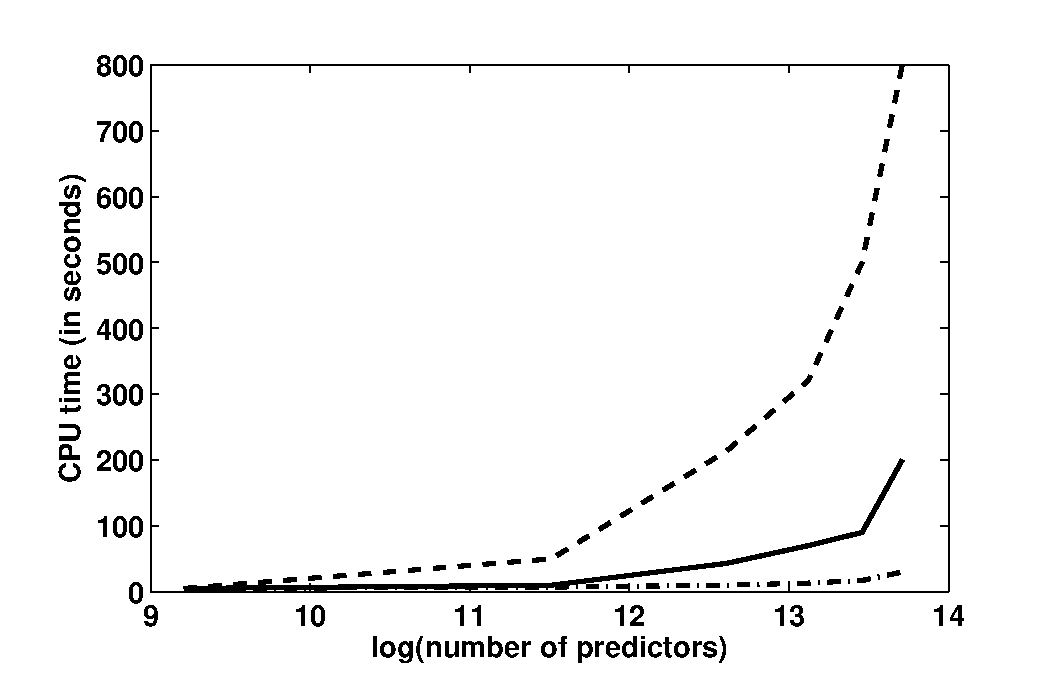
\includegraphics[width=0.8\linewidth]{plotCPU.eps}
%% 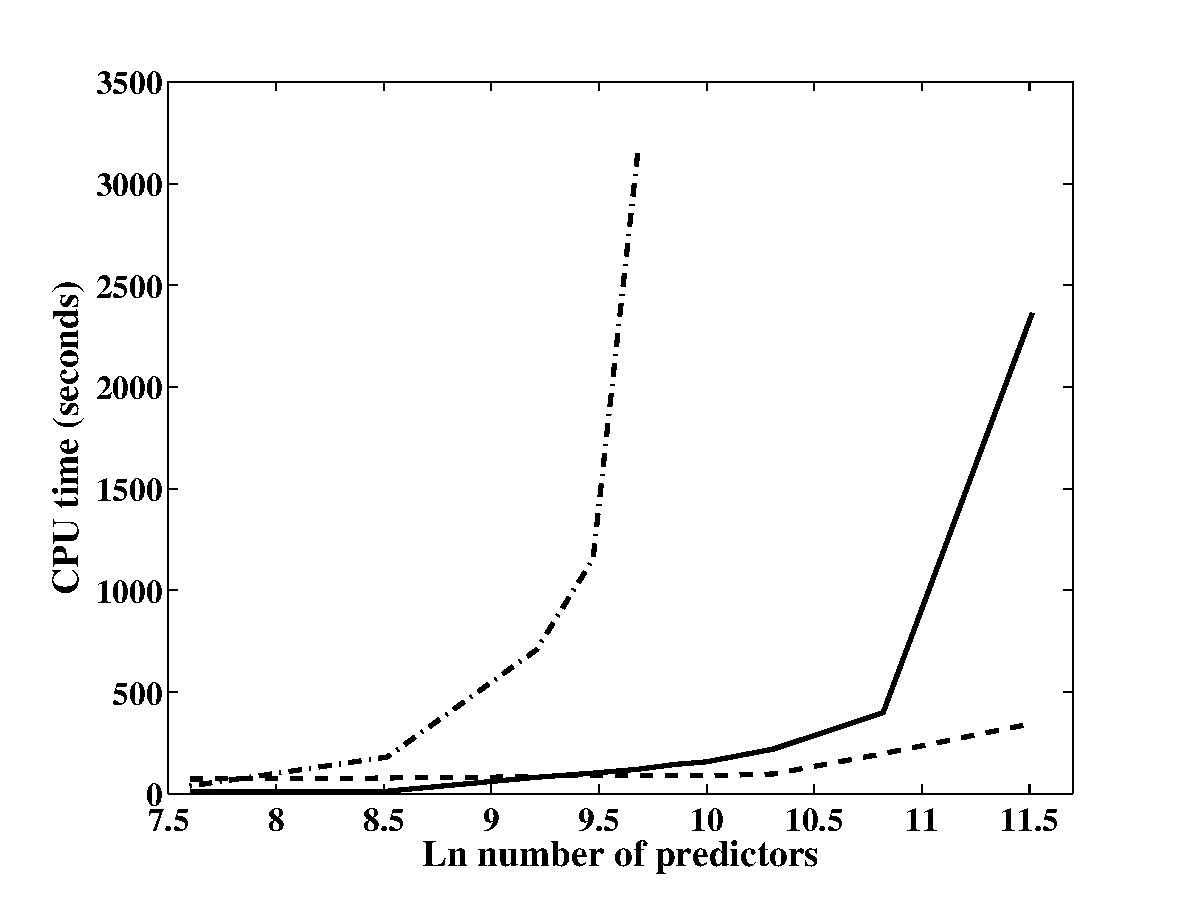
\includegraphics[width=80mm,height=45mm]{Cpu.eps}
%\caption{Elapsed CPU time (in seconds) for a single point prediction based on $200$ observations for MSB (dot-dash), lasso (solid) and CART (dash) for different number of predictors in log-scale.} \label{Cpu}
%\end{figure}
%
%\begin{figure}[h!]
%\centering
%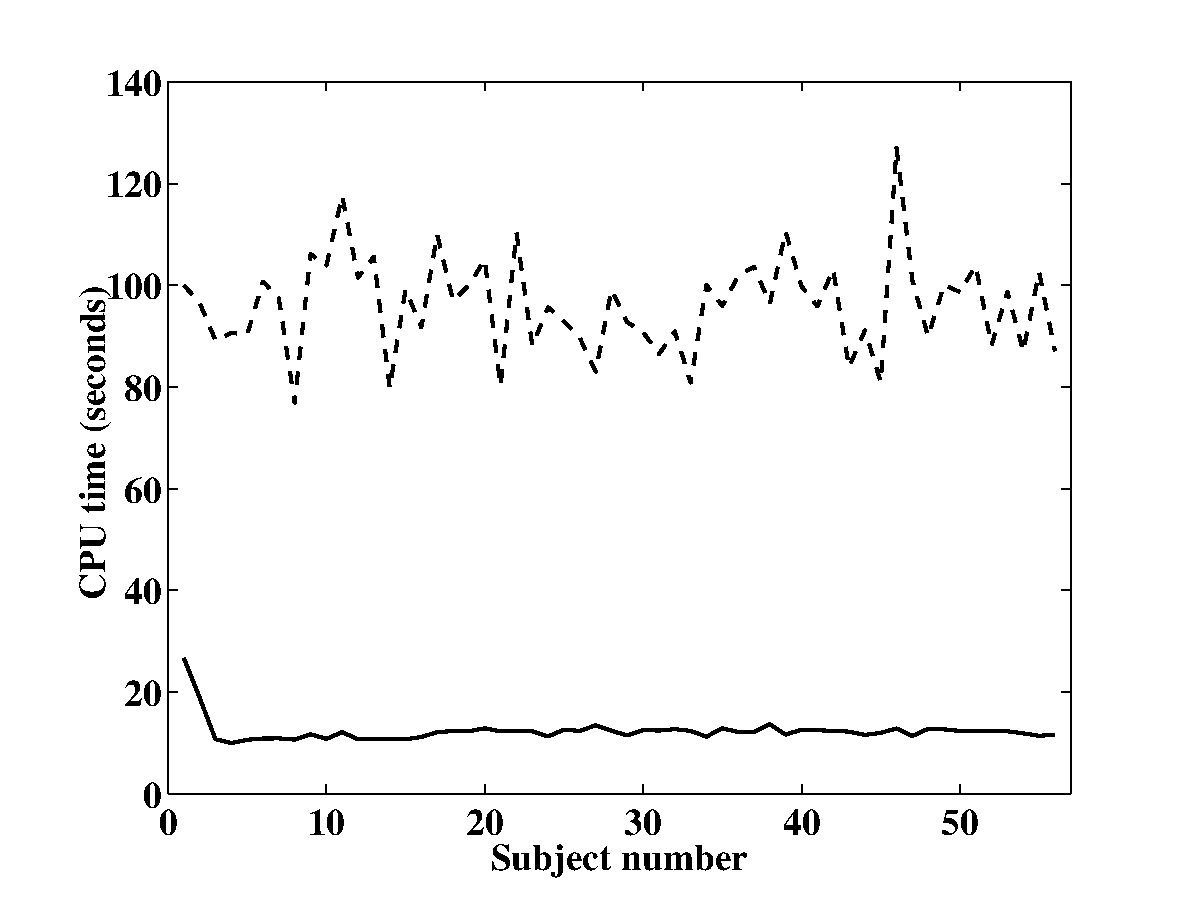
\includegraphics[width=1.0\linewidth]{Time_real2.eps}
%% 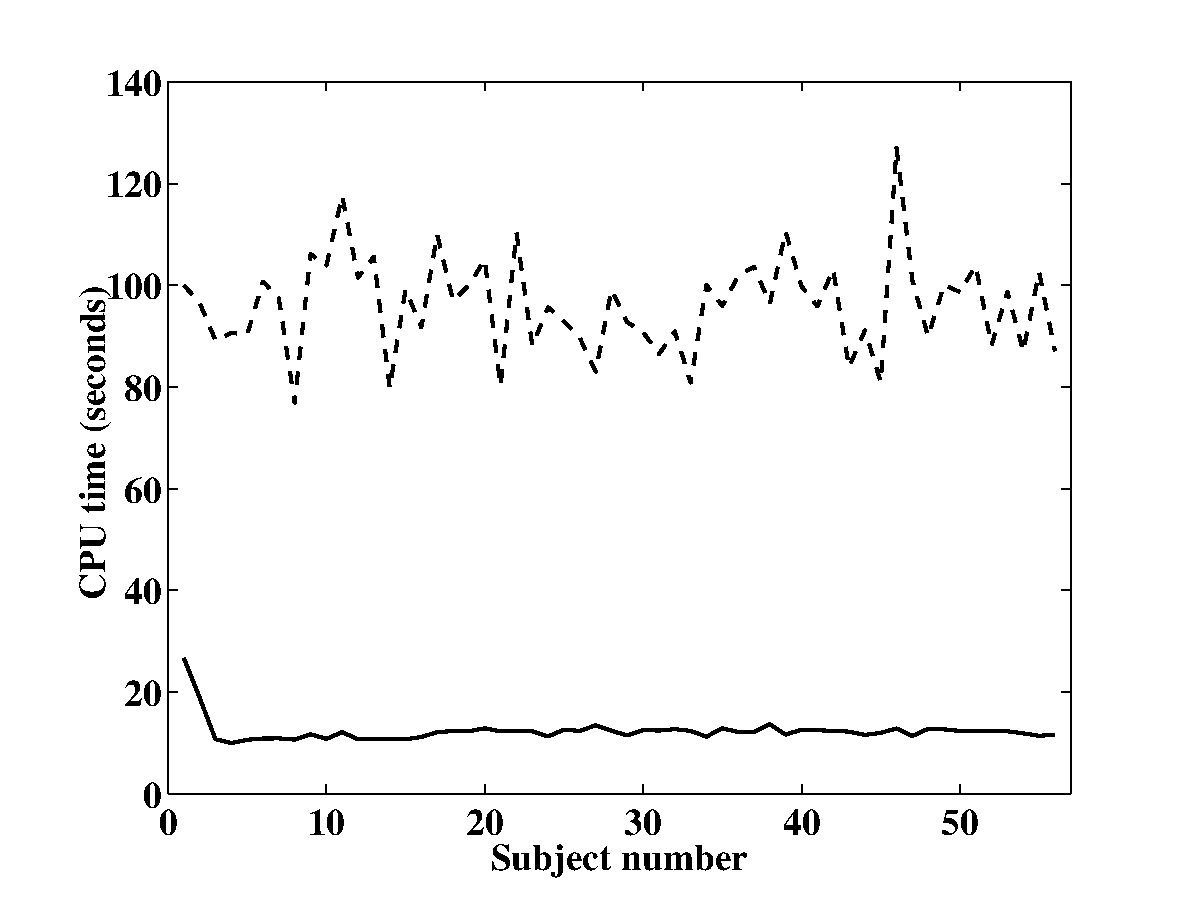
\includegraphics[width=80mm,height=40mm]{Time_real2.eps}
%\caption{Plot of CPU time used to predict each one of the $56$ measurement involved in experiment (2) under MSB (solid) and lasso (dash).} \label{fig:real}
%\end{figure}
%
%\section{Conclusion}
%We have proposed a new model which should lead to substantially improved predictive and computational performance to learn the density of a target variable given a high dimensional vector of predictors. As shown the proposed two stage approach can scale substantially better than other existing algorithms to massive number of features. We have focused on Bayesian MCMC-based methods, but there are numerous interesting directions for ongoing research. Moreover, in addition to better predictive and computational performance, our methods easily extend to parallelized and distributed systems, which we will also explore in future work.


\bibliographystyle{unsrt} 
\bibliography{nipsMSB2} 

\end{document}
